% !TEX root = ../main.tex
\section{Lesson 03 --- 01/10/2026}

\subsection{Cones}

\begin{definition}[Cone]
A set $C \subseteq \R^n$ is a \emph{cone} if, for every $x \in C$ and every $\lambda \ge 0$,
\[
    \lambda x \in C.
\]
\end{definition}

In other words, if $C$ contains a point $x$ different from $0$, then it also contains the whole half-line starting at $0$ and passing through $x$. A cone may be convex or non-convex; here are some examples.

\begin{example}
\leavevmode
\begin{itemize}
    \item $\R_+^n$ is a convex cone.
    \item $\{ x \in \R^2 : x_1 x_2 = 0\}$ is a non-convex cone.
    \item Given a polyhedron $P = \{x \in \R^n : Ax \le b\}$, the \emph{recession cone} of $P$ is
    \[
    \mathrm{rec}(P) = \{d \in \R^n : x+\alpha d \in P \text{ for any } x \in P,\ \alpha \ge 0\},
    \]
    i.e.\ the set of directions along which we never leave the polyhedron. It can be proved that $\mathrm{rec}(P) = \{d : Ad \le 0\}$, so it is a polyhedral cone.
    \item $\{x \in \R^3 : x_3 \ge \sqrt{x_1^2 + x_2^2}\}$ is a non-polyhedral convex cone.
    \item Given $\bar{x} \in \mathrm{cl}(C) \subseteq \R^n$, the \emph{tangent cone} to $C$ at $\bar{x}$ is
    \[
        T_C(\bar{x}) = \Big\{d \in \R^n : \exists \{z_k\} \subset C,\ \exists \{t_k\} > 0,\ z_k \to \bar{x},\ t_k \to 0,\ \lim_{k \to \infty} \frac{z_k - \bar{x}}{t_k} = d\Big\}.
    \]
\end{itemize}
\end{example}

The tangent cone will be the key object in the optimality conditions for constrained problems.

\begin{example}
Let $P_1 = \{x \in \R^2 : x_2 \le x_1,\ x_2 \ge 0\}$, a polyhedral cone: $\mathrm{rec}(P_1) = P_1$ and $T_{P_1}((0,0)) = P_1$.

Let $P_2 = \{x \in \R^2 : x_1 \ge 1,\ x_2 \ge 1,\ x_1 + x_2 \ge 3\}$: then $\mathrm{rec}(P_2) = \{d : d_1 \ge 0,\ d_2 \ge 0\}$ and $T_{P_2}((1,2)) = \{d : d_1 \ge 0,\ d_1 + d_2 \ge 0\}$.
\end{example}

\paragraph{Exercises.}
\begin{itemize}
    \item[1.2] Let $P = \{x : Ax \le b\}$. Prove that $\mathrm{rec}(P) = \{d \in \R^n : Ad \le 0\}$.
    \item[1.3] If $C_1$ and $C_2$ are convex, is $C_1 \cup C_2$ convex?
    \item[1.5] Write $(1,1)$ as a convex combination of $(0,0)$, $(3,0)$, $(0,2)$, $(3,2)$.
\end{itemize}

\subsection{Convex functions}

We now move from sets to functions: convexity of a function is expressed through convexity of a set, its epigraph.

\begin{definition}[Convex function]
Let $C \subseteq \R^n$ be convex. A function $f: \R^n \to \R$ is \emph{convex} on $C$ if, for all $x,y \in C$ and every $\alpha \in [0,1]$,
\[
    f(\alpha y + (1-\alpha)x) \le \alpha f(y) + (1-\alpha)f(x).
\]
When $C = \R^n$ we simply say that $f$ is convex.
\end{definition}

Geometrically, the graph of $f$ between $x$ and $y$ lies below the chord joining $(x, f(x))$ and $(y, f(y))$.

\begin{figure}[htbp]
    \centering
    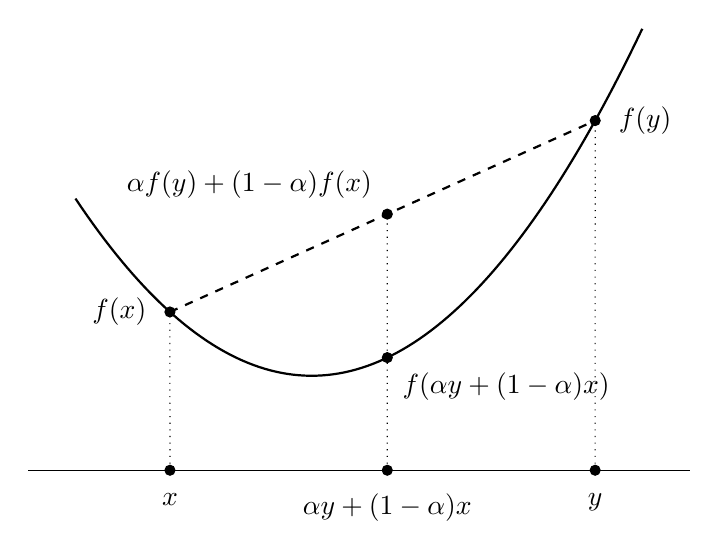
\begin{tikzpicture}[scale=1.2]
        % Asse x (orizzontale)
        \draw (-3, 0) -- (4, 0);

        % Funzione convessa (disegno una parabola f(x) = 0.3*x^2 + 1)
        \draw[thick, domain=-2.5:3.5, samples=100] plot (\x, {0.3*\x*\x + 1});

        % Definisco le coordinate x dei punti per comodità
        \def\xa{-1.5}
        \def\xb{3}
        \def\xc{0.8} % combinazione convessa (il punto in mezzo)

        % Calcolo le coordinate Y dei punti sulla curva
        \coordinate (A) at (\xa, {0.3*\xa*\xa + 1});
        \coordinate (B) at (\xb, {0.3*\xb*\xb + 1});
        \coordinate (C_curve) at (\xc, {0.3*\xc*\xc + 1});

        % Calcolo la coordinata Y del punto sulla corda (linea tratteggiata)
        % Uso la formula dell'interpolazione lineare tra A e B
        \coordinate (C_line) at (\xc, { (0.3*\xa*\xa + 1) + ((0.3*\xb*\xb + 1) - (0.3*\xa*\xa + 1))/(\xb - \xa) * (\xc - \xa) });

        % Disegno la corda (linea tratteggiata)
        \draw[thick, dashed] (A) -- (B);

        % Disegno le linee verticali puntinate
        \draw[dotted] (\xa, 0) -- (A);
        \draw[dotted] (\xb, 0) -- (B);
        \draw[dotted] (\xc, 0) -- (C_line);

        % Disegno i punti sull'asse x e metto le etichette
        \filldraw (\xa, 0) circle (1.5pt) node[below=5pt] {$x$};
        \filldraw (\xb, 0) circle (1.5pt) node[below=5pt] {$y$};
        \filldraw (\xc, 0) circle (1.5pt) node[below=5pt] {$\alpha y + (1-\alpha)x$};

        % Disegno i punti sulla curva e sulla retta e metto le etichette
        \filldraw (A) circle (1.5pt) node[left=5pt] {$f(x)$};
        \filldraw (B) circle (1.5pt) node[right=5pt] {$f(y)$};
        \filldraw (C_curve) circle (1.5pt) node[below right=2pt] {$f(\alpha y + (1-\alpha)x)$};
        \filldraw (C_line) circle (1.5pt) node[above left=2pt] {$\alpha f(y) + (1-\alpha)f(x)$};

    \end{tikzpicture}
    \caption{Example of a convex function.}
    \label{fig:convex_def}
\end{figure}

\begin{theorem}
A function $f:\R^n \to \R$ is convex if and only if the set
\[
    \mathrm{epi}\, f \coloneqq \{(x,y) \in \R^{n} \times \R : y \ge f(x)\},
\]
called the \emph{epigraph} of $f$, is convex.
\end{theorem}

\begin{definition}[Concave function]
Given a convex set $C \subseteq \R^n$, a function $f:\R^n \to \R$ is \emph{concave} on $C$ if $-f$ is convex on $C$.
\end{definition}

Some functions are both convex and concave, like affine functions $f(x) = c^Tx + b$. Every norm $f(x) = \norm{x}$ is convex.

\begin{theorem}[Continuity of convex functions]
Let $f:\R^n \to \R$ be convex on the convex set $C \subseteq \R^n$. Then $f$ is continuous on $\mathrm{ri}(C)$.
\end{theorem}

\subsection{Strictly and strongly convex functions}

\begin{definition}[Strictly convex function]
Given a convex set $C \subseteq \R^n$, $f$ is \emph{strictly convex} on $C$ if
\[
    f(\alpha y + (1-\alpha)x) < \alpha f(y) + (1-\alpha)f(x) \qquad \forall x,y \in C,\ x \ne y,\ \forall \alpha \in (0,1).
\]
\end{definition}

The only difference is that the inequality is strict: a strictly convex function cannot be affine on any segment.

\begin{definition}[Strongly convex function]
Given a convex set $C \subseteq \R^n$, $f$ is \emph{strongly convex} on $C$ if there exists $\tau > 0$ such that, for all $x, y \in C$ and $\alpha \in [0,1]$,
\[
    f(\alpha y + (1-\alpha)x) \le \alpha f(y) + (1-\alpha)f(x) - \frac{\tau}{2}\alpha(1-\alpha)\norm{y-x}_2^2.
\]
\end{definition}

\begin{remark}
Similarly, $f$ is strictly (strongly) concave if $-f$ is strictly (strongly) convex.
\end{remark}

\begin{theorem}
$f$ is strongly convex if and only if there exists $\tau > 0$ such that $f(x) - \frac{\tau}{2}\norm{x}_2^2$ is convex.
\end{theorem}

\begin{remark}
Equivalently, $f$ is strongly convex if and only if $f(x) = \psi(x) + \frac{\tau}{2}\norm{x}_2^2$ for some convex function $\psi$ and some $\tau > 0$.
\end{remark}

\paragraph{Exercise 1.6.} Prove that strongly convex $\Rightarrow$ strictly convex $\Rightarrow$ convex. Do the opposite implications hold?

\subsubsection{First and second order characterizations}

Definitions are hard to check in practice. If $f$ is differentiable we can use derivatives. Assume from now on that $C \subseteq \R^n$ is open and convex.

\begin{theorem}[First order condition]
Let $f$ be continuously differentiable on $C$. Then $f$ is convex on $C$ if and only if
\[
    f(y) \ge f(x) + (y-x)^T \nabla f(x) \qquad \forall x,y \in C.
\]
\end{theorem}

The function $y \mapsto f(x) + (y-x)^T\nabla f(x)$ is the tangent plane to $f$ at $x$, so the theorem says that $f$ is convex if and only if it always lies above its tangent planes (the first-order approximation is a global underestimator).

The same idea characterizes strict and strong convexity.

\begin{theorem}
Let $f$ be continuously differentiable on $C$.
\begin{itemize}
    \item $f$ is strictly convex on $C$ if and only if
    \[
        f(y) > f(x) + (y-x)^T \nabla f(x) \qquad \forall x,y \in C,\ x \ne y.
    \]
    \item $f$ is strongly convex on $C$ if and only if there exists $\tau > 0$ such that
    \[
        f(y) \ge f(x) + (y-x)^T \nabla f(x) + \frac{\tau}{2}\norm{y-x}_2^2 \qquad \forall x,y \in C.
    \]
\end{itemize}
\end{theorem}

If $f$ is twice continuously differentiable we can look at the Hessian.

\begin{theorem}[Second order conditions]
Let $f$ be twice continuously differentiable on $C$.
\begin{itemize}
    \item $f$ is convex on $C$ if and only if $\nabla^2 f(x)$ is positive semidefinite for all $x \in C$, i.e.
    \[
        v^T \nabla^2 f(x) v \ge 0 \quad \forall v \in \R^n,\ \forall x \in C,
    \]
    or, equivalently, the eigenvalues of $\nabla^2 f(x)$ are non-negative for all $x \in C$.
    \item If $\nabla^2 f(x)$ is positive definite for all $x \in C$, then $f$ is strictly convex on $C$.
    \item $f$ is strongly convex on $C$ if and only if there exists $\tau > 0$ such that $\nabla^2 f(x) - \tau I_n$ is positive semidefinite for all $x \in C$, i.e.
    \[
        v^T \nabla^2 f(x) v \ge \tau\norm{v}_2^2 \quad \forall v \in \R^n,\ \forall x \in C,
    \]
    or, equivalently, the eigenvalues of $\nabla^2 f(x)$ are greater than or equal to $\tau$ for all $x \in C$.
\end{itemize}
\end{theorem}

\subsubsection{Examples and exercises}

\begin{example}
Let $f: \R \to \R$.
\begin{itemize}
    \item $f(x) = e^{px}$, $p \ne 0$, is strictly convex on $\R$ but not strongly convex.
    \item On $C = \R_+ \setminus \{0\}$: $f(x) = x^p$ is strictly convex if $p > 1$ or $p < 0$, and strictly concave if $0 < p < 1$; $f(x) = \log x$ is strictly concave but not strongly concave.
\end{itemize}
Let $f: \R^n \to \R$.
\begin{itemize}
    \item $f(x) = \norm{x}$ is convex but not strictly convex.
    \item $f(x) = \max\{x_1, \dots, x_n\}$ is convex but not strictly convex.
\end{itemize}
\end{example}

\paragraph{Exercises.}
\begin{itemize}
    \item[1.7] Prove that $f(x) = \norm{x}$ is convex, whatever the norm.
    \item[1.8] Prove that if $f$ is convex, $x^1, \dots, x^k \in C$ and $\alpha_1, \dots, \alpha_k \in (0,1)$ with $\sum_i \alpha_i = 1$, then $f(\sum_i \alpha_i x^i) \le \sum_i \alpha_i f(x^i)$. (Hint: follow the proof of the lemma on convex combinations.)
    \item[1.9] Prove that $f(x_1, x_2) = \frac{1}{x_1 x_2}$ is convex on $\{x \in \R^2 : x_1, x_2 > 0\}$.
    \item[1.10] Analyse the convexity properties of $f(x_1,x_2,x_3) = 2x_1^2 + 2x_2^2 + x_3^2 + 3x_1x_2 + x_2x_3 - 6x_1 - 4x_2 - 3x_3$.
    \item[1.11] If $f_1$ and $f_2$ are convex, is the product $f_1 f_2$ convex?
\end{itemize}
